\documentclass[12pt,letterpaper]{article}
\usepackage{fullpage}
\usepackage[top=2cm, bottom=4.5cm, left=2.5cm, right=2.5cm]{geometry}
\usepackage{amsmath,amsthm,amsfonts,amssymb,amscd}
\usepackage{lastpage}
\usepackage{enumerate}
\usepackage{fancyhdr}
\usepackage{mathrsfs}
\usepackage{xcolor}
\usepackage{graphicx}
\usepackage{listings}
\usepackage{hyperref}
\usepackage{fontspec,xunicode,xltxtra}
\usepackage{geometry}
\usepackage{xeCJK}
\usepackage{caption}
\usepackage{hyperref}
\usepackage{graphicx}
\setCJKmainfont{KaiTi}
%\setmainfont{Times New Roman}
\setCJKfamilyfont{hei}{SimHei}                                    %黑体  hei
\newcommand{\hei}{\CJKfamily{hei}}      

\hypersetup{%
  colorlinks=true,
  linkcolor=blue,
  linkbordercolor={0 0 1}
}
 
\renewcommand\lstlistingname{Algorithm}
\renewcommand\lstlistlistingname{Algorithms}
\def\lstlistingautorefname{Alg.}
\usepackage{algorithm}
\usepackage{algorithmicx}
\usepackage{algpseudocode}
\renewcommand{\algorithmicrequire}{\textbf{Input: }}
\renewcommand{\algorithmicensure}{\textbf{Output: }}

\lstdefinestyle{Python}{
    language        = Python,
    frame           = lines, 
    basicstyle      = \footnotesize,
    keywordstyle    = \color{blue},
    stringstyle     = \color{green},
    breaklines      = true
    commentstyle    = \color{red}\ttfamily
}
\lstset{escapechar=@,style=Python}

\setlength{\parindent}{0.0in}
\setlength{\parskip}{0.05in}

% Edit these as appropriate
\newcommand\course{现代信息网络技术}
\newcommand\hwnumber{3}                  % <-- homework number
\newcommand\NetIDa{罗雁天}           % <-- NetID of person #1
\newcommand\NetIDb{2018310742}           % <-- NetID of person #2 (Comment this line out for problem sets)

\pagestyle{fancyplain}
\headheight 35pt
\lhead{\NetIDa}
\lhead{\NetIDa\\\NetIDb}                 % <-- Comment this line out for problem sets (make sure you are person #1)
\chead{\textbf{\Large Homework \hwnumber}}
\rhead{\course \\ \today}
\lfoot{}
\cfoot{}
\rfoot{\small\thepage}
\headsep 1.5em

\begin{document}
\section{问题描述}
根据RFC6052,在课程的虚拟机上写一个程序(用bash、 C、 python等均可),给定任意IPv4地址和 /40的任意IPv6前缀,输出结果。

\section{算法描述}
如图\ref{algo}所示,对于题目要求的问题,我们只需关注红框所在的行即可。
\begin{figure}[!h]
	\centering
	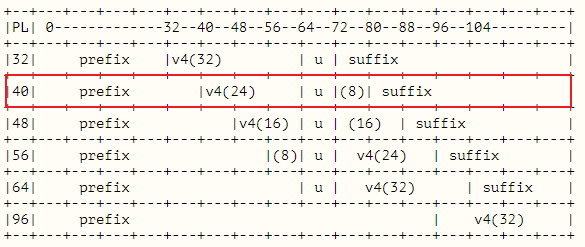
\includegraphics[width=\linewidth]{algo}
	\caption{\label{algo}IPv4地址和IPv6前缀生成IPv6地址示意图}
\end{figure}

对于给定任意IPv4地址和 /40的任意IPv6前缀,我们采用Algorithm \ref{alg1}计算生成的IPv6地址。
\begin{algorithm}[H]
	\caption{\label{alg1}IPv4地址和/40的任意IPv6前缀生成IPv6地址算法}
	\begin{algorithmic}[1]
		\Require /40的任意IPv6前缀,IPv4地址
		\Ensure IPv6地址
		\State 初始化IPv6地址为128bit的全0字符串$x$
		\State $x[0:39]=$IPv6前缀(5个字节(40bit))
		\State $x[40:55]=$IPv4地址的前3个字节(24bit)
		\State $x[64:71]=0$
		\State $x[72:79]=$IPv4地址的第4个字节(8bit)
		\State $x[80:127]$可以任意设置后缀,在本次实验中全设置为0
	\end{algorithmic}
\end{algorithm}

\section{实验结果}
本次实验使用$python3.7$完成,由于课程虚拟机上没有安装$python3.7$,因此首先在$ee01$虚拟机上安装了anaconda3。代码文件为``main.py'',使用如下方式执行:
\begin{lstlisting}
python main.py ipv4_address ipv6_prefix
\end{lstlisting}

测试了几个转换结果,列表如下:
\begin{table}[!h]
	\centering
	\caption{\label{res}实验结果统计表}
	\begin{tabular}{|c|c|c|}
		\hline
		prefix & IPv4 address & IPv6 address \\
		\hline
		2001:db8:100::/40 & 192.0.2.33 & 2001:db8:1c0:2:21:: \\
		\hline
		2402:f000:100::/40 & 166.111.4.100 & 2402:f000:1a6:6f04:64:: \\
		\hline
		2001:db8:ab00::/40 & 192.168.1.101 & 2001:db8:abc0:a801:65:: \\
		\hline
	\end{tabular}
\end{table}
\end{document}
